\chapter{State of the Art}

\section{SR Design \& Implementation}
Diffusion \autocite{NEURIPS2020_4c5bcfec} models have recently overtaken GAN \autocite{NIPS2014_5ca3e9b1} models in the state-of-the-art of generative image methodologies \autocite{10081412}. While GANs have been extensively used in image super-resolution \autocite{9044873}, they are unstable due to their very delicate training process. Diffusion models, which are also probabilistic models drawing results from a likelihood distribution, have proven to be easier to train and deliver better results, surpassing other methodologies in many reconstruction metrics \autocite{saharia2021image}. This development has also been noticed in the remote sensing community, with recent super-resolution papers switching to diffusion-based SR methodologies \autocite{rs14194834, 10057005, 103389fmars20231211981}.

\begin{figure}[H]
    \caption{\doublespacing \\ \textit{Pixel-space (above) and latent-space (below) diffusion models.}} 
    \centering
    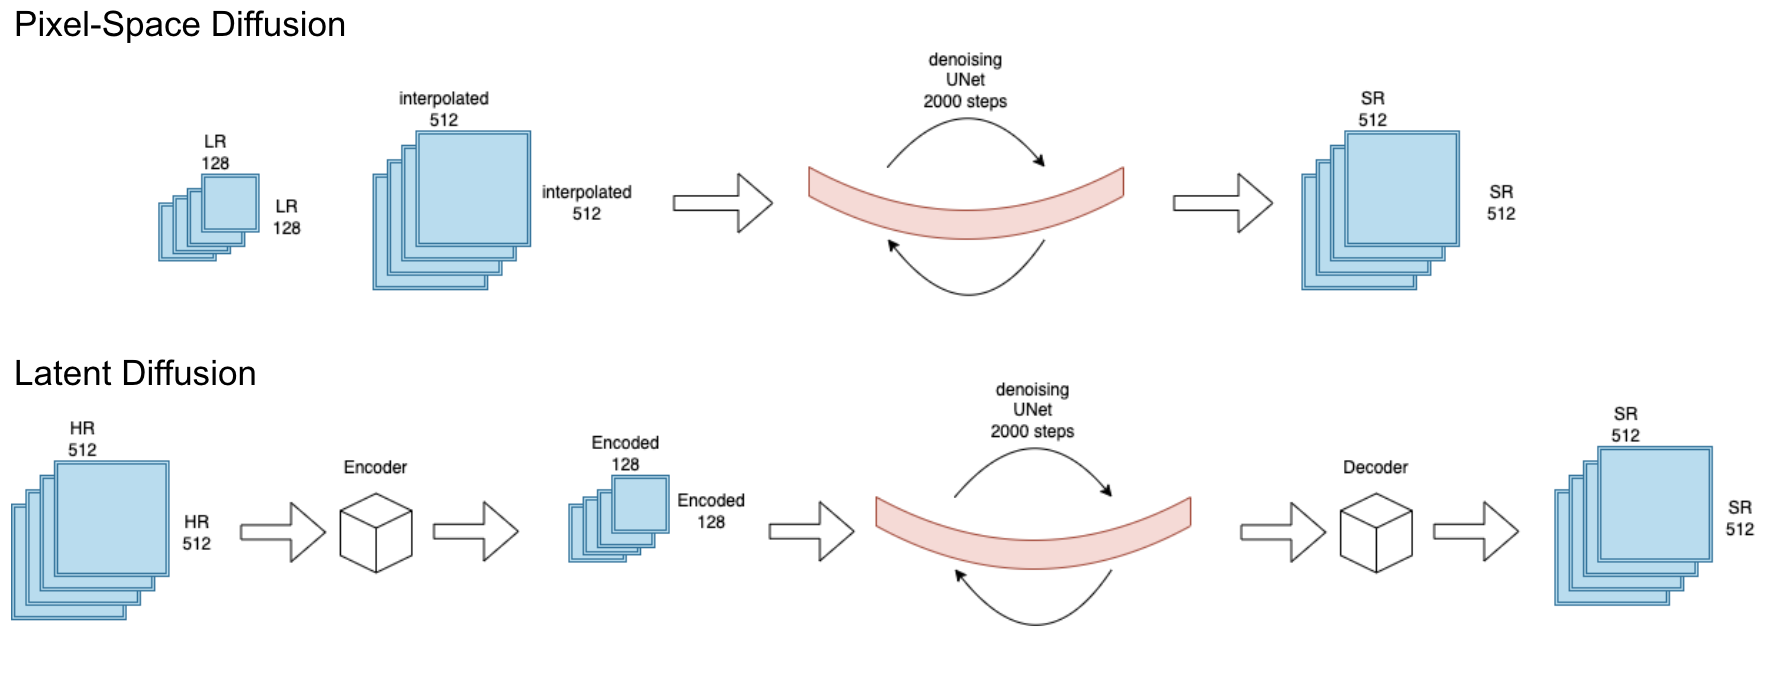
\includegraphics[width=1\linewidth]{images/lat_px_dif.png}
    \begin{justify}
        \textit{Note.} Pixel-space (above) and latent-space (below) diffusion models.
    \end{justify}                    
    \label{fig:pixel_latent_space}
\end{figure}

\subsection{Latent-Diffusion vs Pixel-Space Diffusion}

Most SR models found in the literature use pixel-space diffusion (see Figure \ref{fig:pixel_latent_space}, top). In this workflow, the $LR$ image is interpolated to the desired size. The denoising U-Net, which is cycled through \textit{n} times, removing a small amount of noise in each iteration. This method is very computationally expensive, since each image that needs to be super-resoluted has to pass many times through the whole network to receive the output. In general, 500 to 2000 of these iterations are used.

Latent diffusion models on the other hand perform the computationally expensive denoising steps on a lower-dimension representation of the input image (see fig. \ref{fig:pixel_latent_space}, bottom). A separate network, the autoencoder, generates a latent space and smaller than the original input space and therefore makes the denoising step much faster. After the denoising, the image is decoded and inflated again to the original desired dimensionality of the SR product. It has been shown that performing latent diffusion significantly reduces computational requirements while preserving the powerful SR capabilities of diffusion models \autocite{rombach2022highresolution}.


\subsection{Codebase}

Several code-bases related to super-resolution (SR) models have been developed and are available for exploration and implementation (see fig. \ref{fig:codebase}). Among them, two unofficial implementations of the SR3 model \autocite{saharia2021image} stand out: one hosted on \href{https://github.com/Janspiry/Image-Super-Resolution-via-Iterative-Refinement}{GitHub by Janspiry} and another by \href{https://github.com/KiUngSong/Generative-Models/tree/main/SR3}{KiUngSong}. While these repositories provide valuable insights into SR3’s functionality, they focus on pixel-space diffusion and have received feedback from the community regarding certain design choices and limitations in code quality and expandability. Additionally, these implementations tend to yield medium-quality results.


\begin{figure}[H]
    \caption{\doublespacing \\ \textit{Codebases in use.}} 
    \centering
    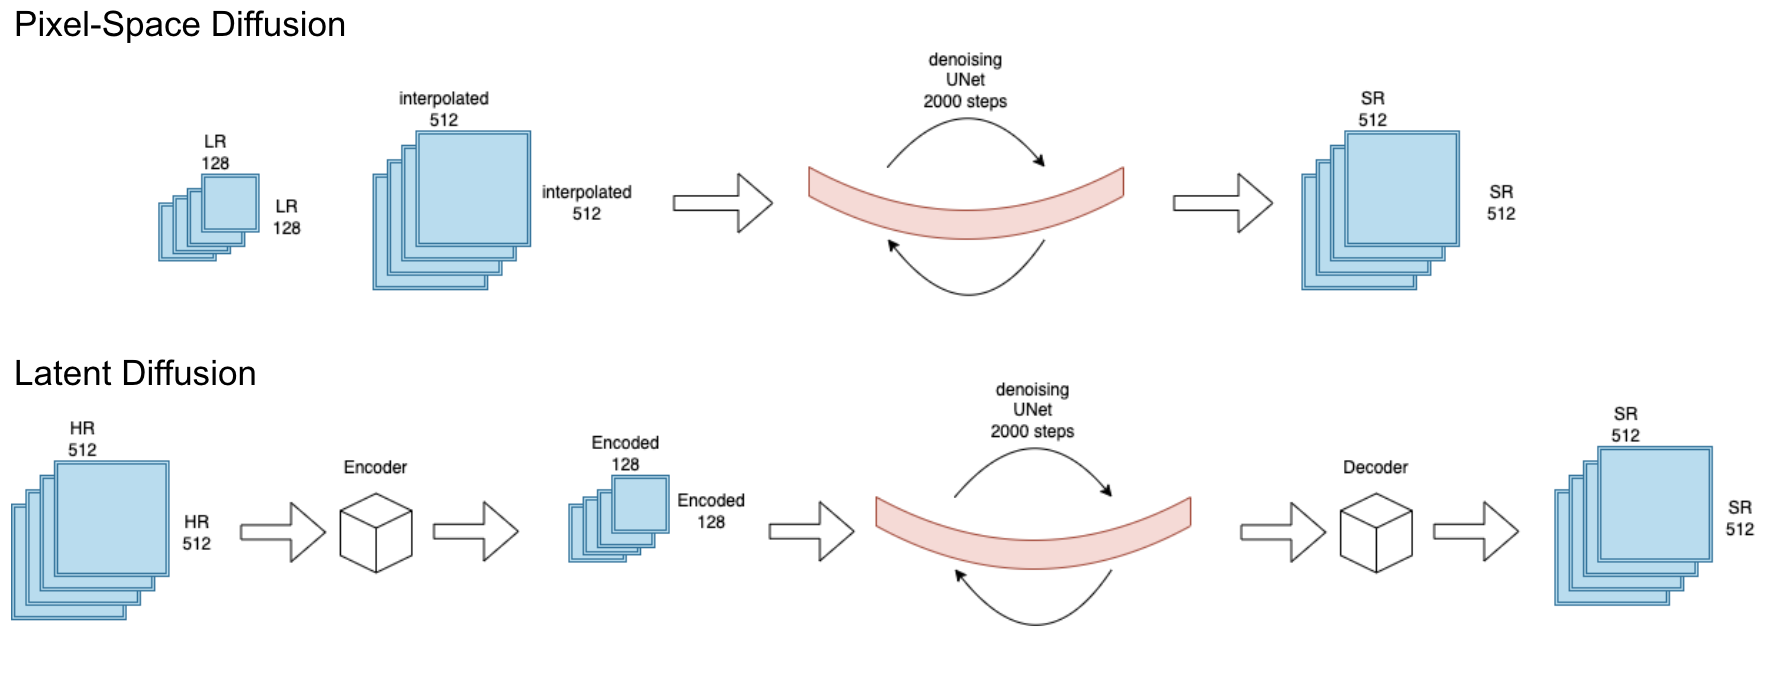
\includegraphics[width=1\linewidth]{images/lat_px_dif.png}
    \begin{justify}
        \textit{Note.} Codebases in use.
    \end{justify}                    
    \label{fig:codebase}
\end{figure}

Another noteworthy resource is the \href{https://github.com/mikonvergence/DiffusionFastForward}{DiffusionFastForward} repository, which serves as a clear tutorial-like implementation for both pixel-space and latent-space diffusion models. However, it is relatively simple and heavily reliant on external repositories, limiting its scalability and modifiability. Despite its simplicity, it offers a good understanding of the core diffusion strategies for SR.

Finally, the \href{https://github.com/mikonvergence/DiffusionFastForward}{latent-diffusion} repository, the official code-base of the highly successful latent-diffusion model \autocite{rombach2022highresolution}, offers a comprehensive solution that encompasses various tasks such as unconditional image generation, text-prompt-based image generation, inpainting, and super-resolution. This repository is known for its versatility and well-organized structure, making it highly adaptable for further modifications and expansions. The availability of pre-trained checkpoints provided by the authors also allows for immediate demonstration of the model’s strong capabilities, positioning it as a leading resource for super-resolution projects.


\subsection{Autoencoder}

The autoencoder under consideration is designed to compress the spatial dimension by a factor of 4, reducing tensors from \textit{4$\times$512$\times$512} to \textit{4$\times$128$\times$128} before decoding them back to their original dimensions. This approach is inspired by the \textit{latent-diffusion} repository, as described in \autocite{rombach2022highresolution}. Ideally, such encoding and decoding processes aim to preserve image quality. Beyond reconstruction metrics, the latent space produced by the autoencoder plays a crucial role in super-resolution, as the denoising occurs after the encoder. This type of autoencoder has been effectively utilized in various applications, as demonstrated by the latent diffusion model and its adaptations in prior research \autocite{esser2021taming}.

In this context, models are often trained independently from the denoising U-Net, using a combination of perceptual LPIPS and a GAN component. The GAN component typically employs a classifier that distinguishes between real images and reconstructed images, where the output logits are combined with the perceptual loss and then back-propagated through the autoencoder. The LPIPS metric \autocite{zhang2018unreasonable} is widely used in computer vision tasks, simulating human visual perception to return a similarity score between two images. Since LPIPS is based on a VGG network \autocite{simonyan2015deep} and is primarily trained on RGB data, extending it to handle more than 3 bands presents challenges, especially for 4-band models like RGB-NIR. In such cases, a common workaround involves selecting 3 bands at random during each training step and feeding them into the LPIPS model. Although unconventional, this method has been validated, as random permutations of the 4-band tensor into 3 bands have shown no significant loss in LPIPS accuracy. Figure \ref{fig:lpips_permutation} demonstrates that the LPIPS boxplot results for 200 interpolated LR-HR image pairs remain consistent, even when using spectral band combinations that were not part of the original training, thus supporting the viability of this approach.


\begin{figure}[H]
    \caption{\doublespacing \\ \textit{LPIPS boxplots for all possible 3 band permutations from the 4 band tensors.}} 
    \centering
    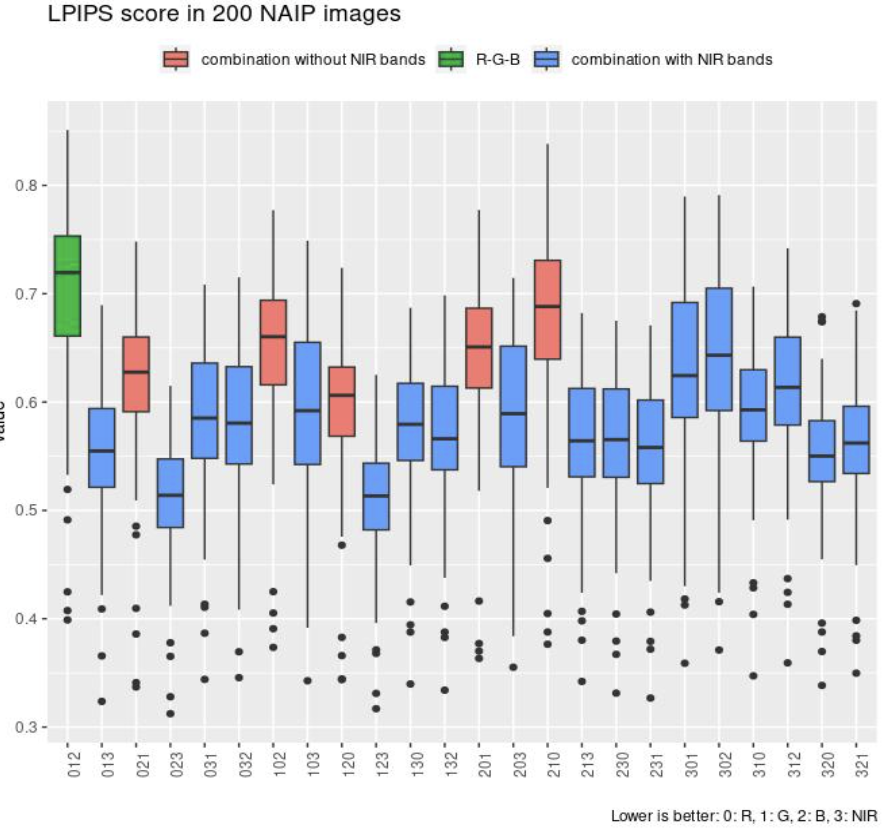
\includegraphics[width=1\linewidth]{images/lpips_permutation.png}
    \begin{justify}
        \textit{Note.} LPIPS boxplots for all possible 3 band permutations from the 4 band tensors.
    \end{justify}                    
    \label{fig:lpips_permutation}
\end{figure}


\begin{figure}[H]
    \caption{\doublespacing \\ \textit{Minimum (light red), mean (orange), standard deviation (green), and maximum (blue) of the encoded value ranges.}} 
    \centering
    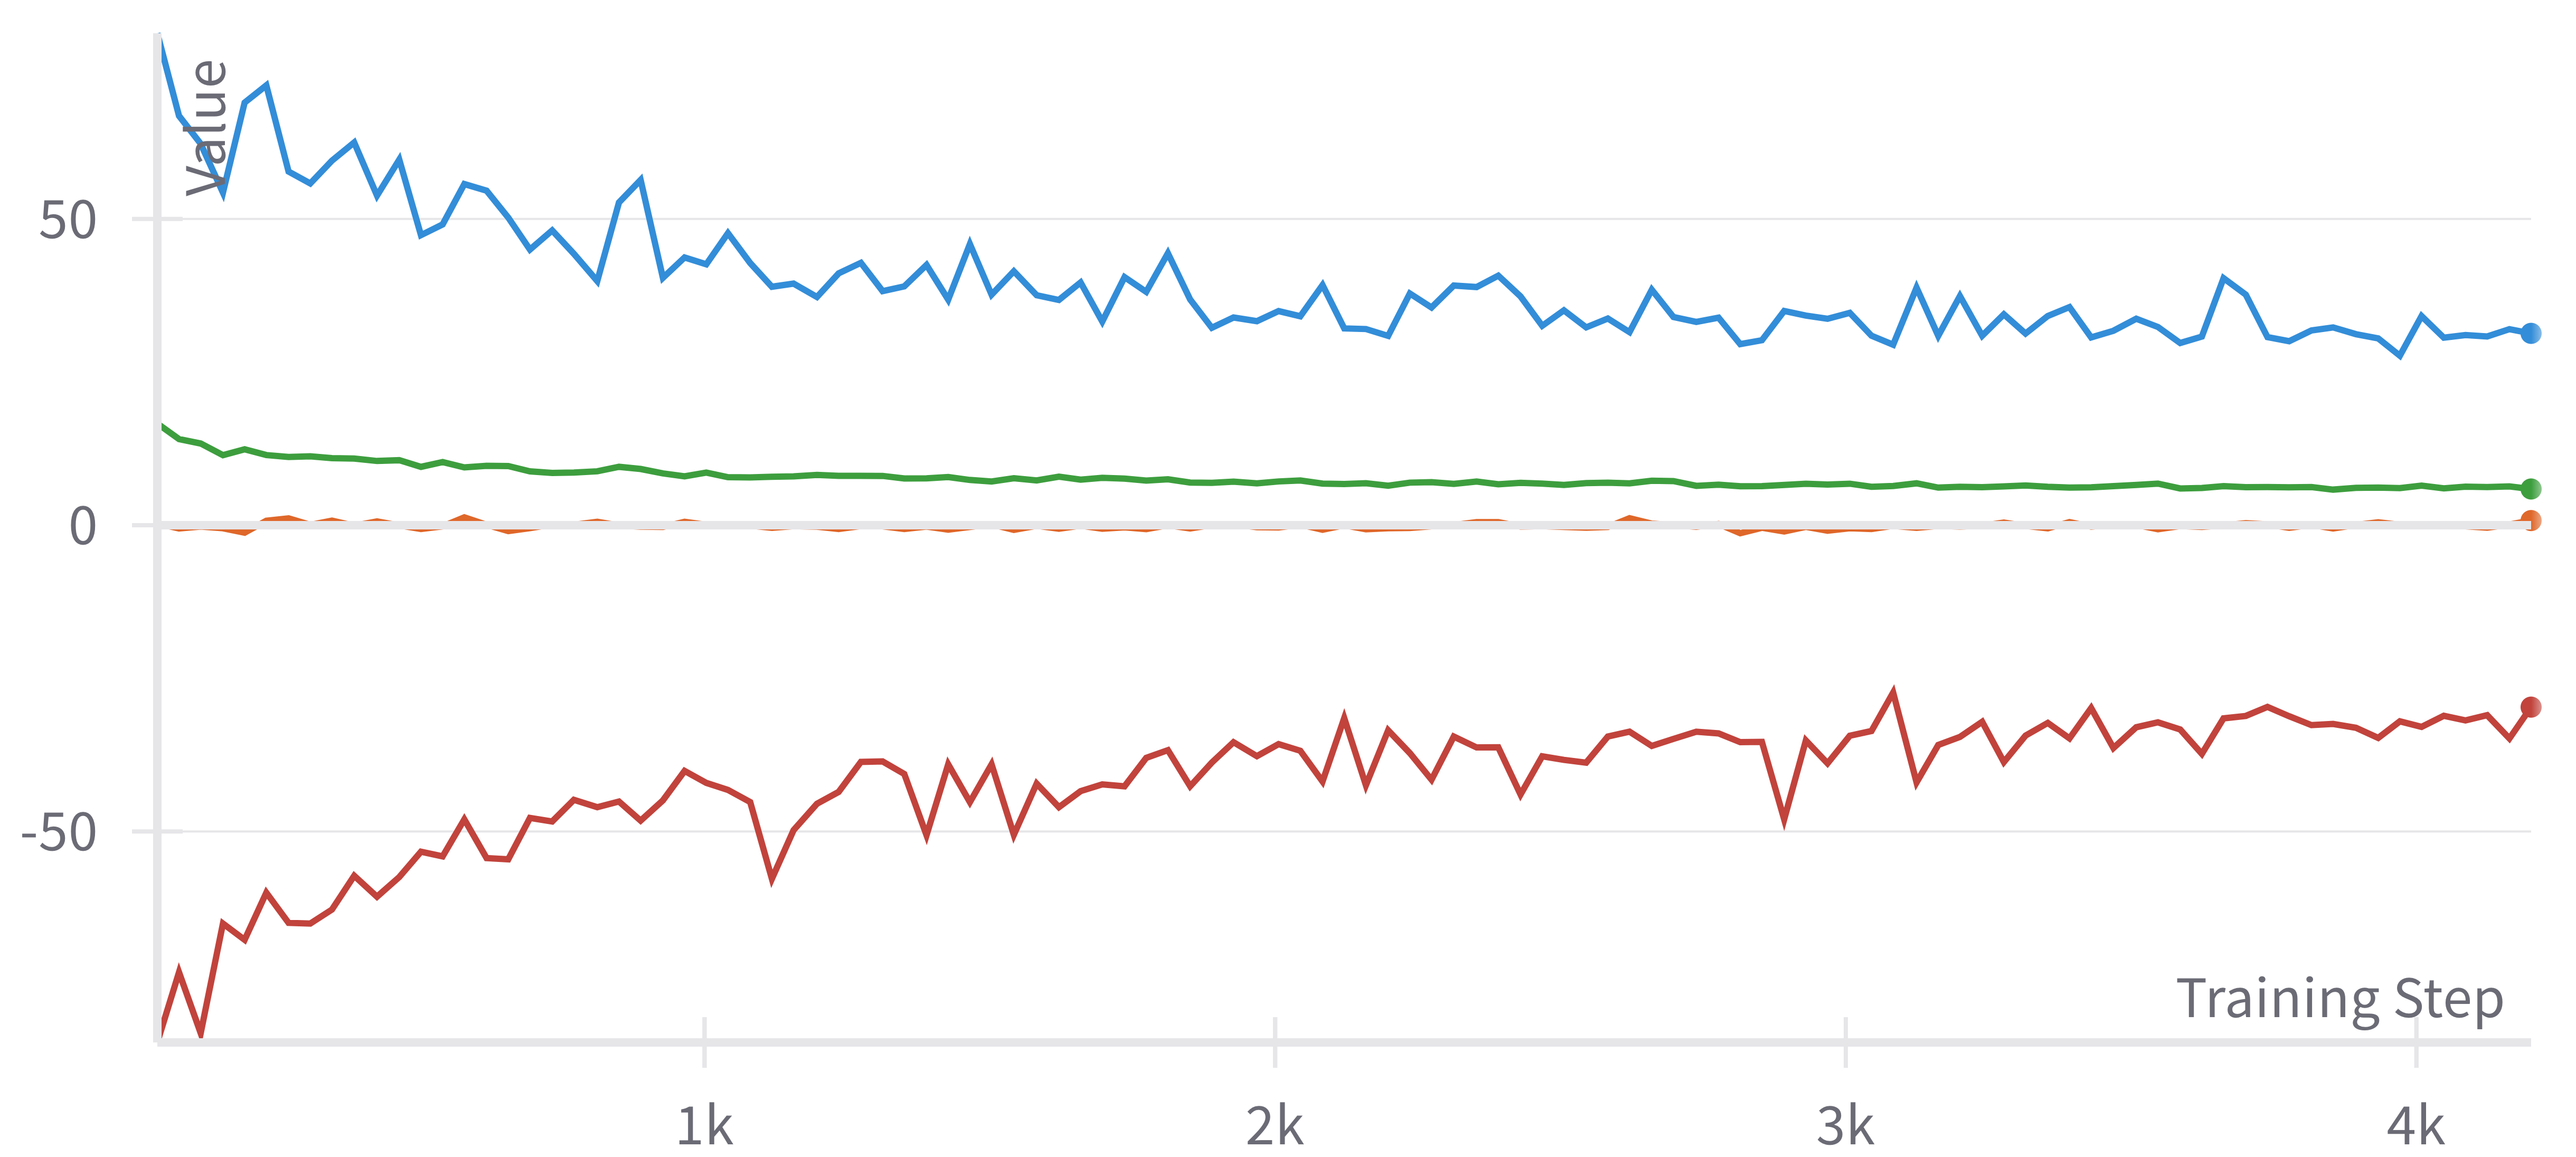
\includegraphics[width=1\linewidth]{images/simon/ae_distr_enc.png}
    \begin{justify}
        \textit{Note.} Minimum (light red), mean (orange), standard deviation (green), and maximum (blue) of the encoded value ranges during AE training. While we want the value range to be similar to the input images, if the value range is compressed too much we lose the ability to recover the images accurately.
    \end{justify}                    
    \label{fig:ae_distr_enc}
\end{figure}


Additionally, an autoencoder with Kullback-Leibler regularization is used to ensure that the latent space closely mirrors the input image distribution. This regularization penalizes the encoder when the encoded image strays too far from the original image distribution, which is particularly crucial during the inference stage, where the encoding process is skipped, and the image is directly denoised and super-resolved from \textit{128$\times$128} $LR$ dimensions to \textit{512$\times$512} $HR$ dimensions in the decoder. Maintaining the encoded image distribution as close as possible to the $LR$ image (minus the noise) is key to achieving high-quality results.

Balancing the regularization of the encoded values is essential to ensuring that the encoded image remains similar to the input, while also capturing enough variation. Over-regularization, such as reducing the extremes or standard deviation of the latent space too much, can degrade reconstruction quality (see \autoref{fig:ae_distr_enc}). Empirical evidence suggests that a standard deviation around 5 strikes the optimal balance. By leveraging 32-bit floating-point numbers, this process effectively translates some of the high-resolution spatial complexity into numerical representation. Without this complexity, the reconstruction quality suffers.

Training the autoencoder (AE) is a delicate process. While the decoder's output converges rapidly—visually reconstructing the input image quite quickly—the resulting model checkpoint is not immediately ready for integration into the super-resolution (SR) workflow. The GAN component requires a warm-up period before its loss is weighted, and the regularization needs time to take effect. Furthermore, the autoencoder requires a large amount of satellite imagery data for training due to its size, with over 72 million parameters.

\begin{figure}[H]
    \caption{\doublespacing \\ \textit{Visualization of the original image, the encoded image, and the recovered image (f.l.t.r.).}} 
    \centering
    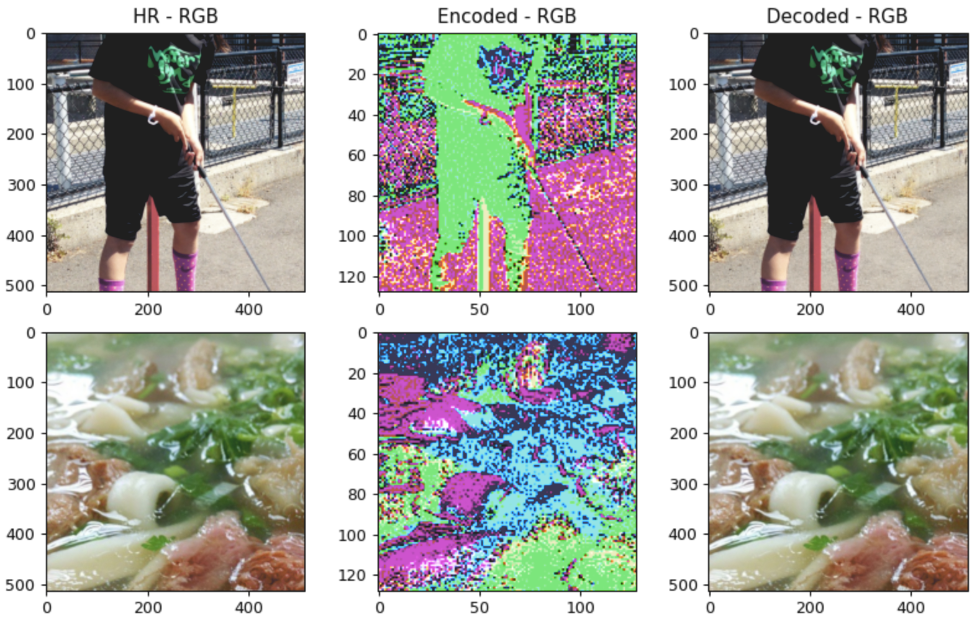
\includegraphics[width=1\linewidth]{images/autoencoder.png}
    \begin{justify}
        \textit{Note.} Visualization of the original image, the encoded image, and the recovered image (f.l.t.r.).
    \end{justify}                    
    \label{fig:autoencoder}
\end{figure}


\autoref{fig:autoencoder} illustrates that while the image is faithfully reconstructed, the latent space might not yet be optimized for SR with the U-Net. Extensive training, careful learning rate schedules, and warm-up periods, along with latent space regularization, are required to avoid this issue.

\subsection{Denoising UNet}
The denoising probabilistic model is designed to iteratively predict a denoised version of the input image by learning the input data distribution. This process can be described as a Markov chain, where each timestep determines both preceding and following states. By learning the distribution $p(x)$ of the input data, the model is able to reverse the chain and produce denoised images. The training minimizes the variational lower bound on the log-likelihood of the data under the model, penalizing outputs that fall on the lower end of the probability scale with respect to the target distribution.

The denoising model uses a U-Net backbone, augmented with noise-adding functions that handle both the addition and removal of normally distributed noise. Since the autoencoder handles a 4x upscaling, the model can be conditioned on the $LR$ image. Therefore, instead of starting from a pure noise image, the denoising process begins with the $LR$ image and progressively removes noise, recovering lost quality before the image is upscaled by the autoencoder. This approach has been successfully demonstrated by \autocite{rombach2022highresolution} for various tasks, such as conditional and unconditional image generation, inpainting, style transfer, and super-resolution. In this workflow, the U-Net is conditioned on the $LR$ image in the original spectral domain, specifically in the RGB-NIR color space (see \autoref{fig:encLR_schema}).

\subsubsection{UNet Adaptations}
As the autoencoder's sampling process expects a distribution similar to that of its own training (see \autoref{fig:ae_distr_enc}), the U-Net implicitly learns to transform the input spectral distribution into the encoded spectral distribution. Although this transformation does not affect spatial feature reconstruction, it does impact the spectral consistency of the SR image. To mitigate this, we interpolate the $LR$ image to the same dimensions as the $HR$ image before encoding. This change relieves the U-Net from the burden of learning the mapping between the two spectral domains (\autoref{fig:encLR_schema}). During training, this results in a conditioning that concatenates the noise-encoded $HR$ tensor with the same-size $LR$ image, rather than mixing spectral domains. At inference, the encoded $HR$ image is replaced by only the noise tensor from the scheduler.

Experimentation demonstrates that the interpolated $LR$ image can be easily encoded and decoded by the autoencoder, even though the AE was trained on $HR$ images (\autoref{fig:encLRint_demo}). Although this adds an additional pass through the AE, it does not significantly increase processing time during training or inference.

\begin{figure}[H]
    \caption{\doublespacing \\ \textit{Schema of the changes to the UNet SR workflow.}} 
    \centering
    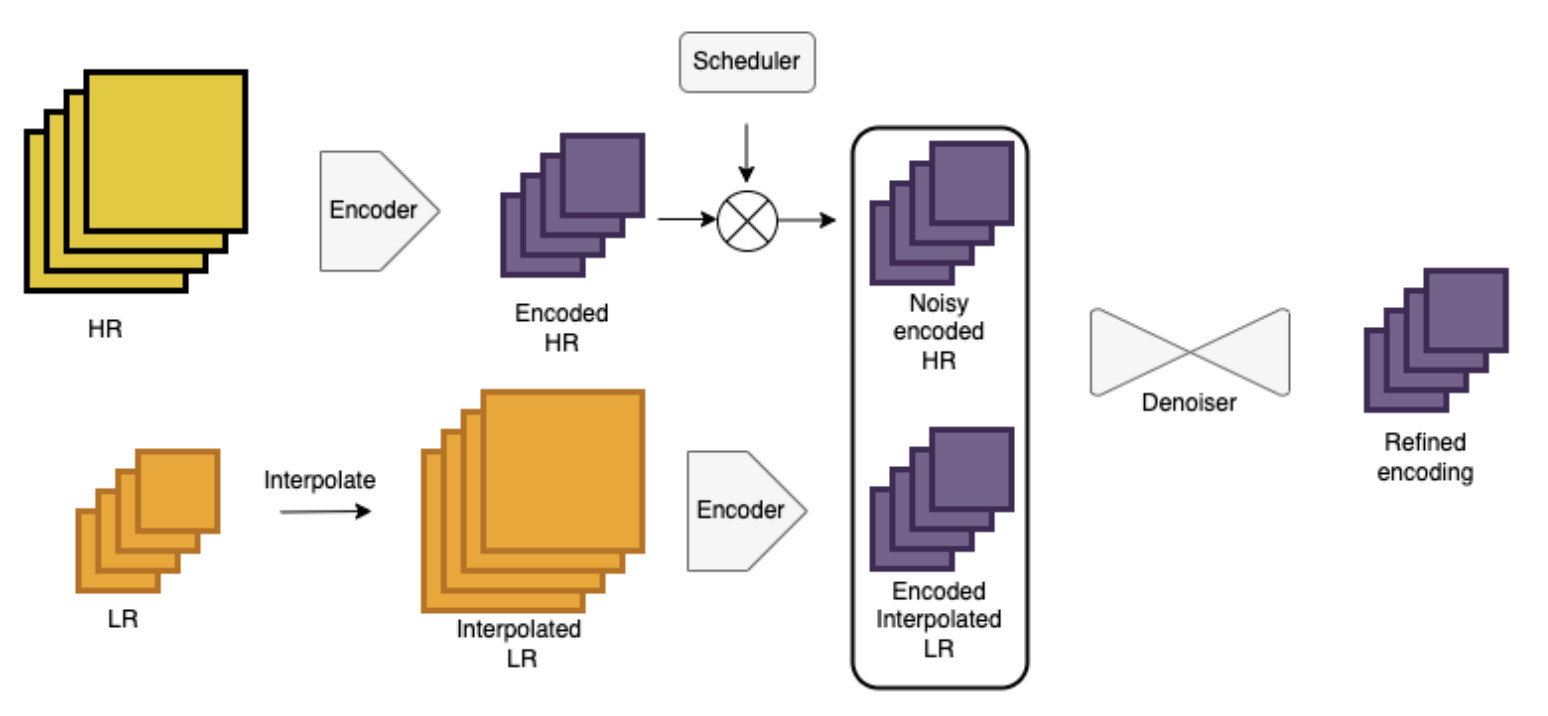
\includegraphics[width=1\linewidth]{images/simon/encLR_schema.png}
    \begin{justify}
        \textit{Note.} Schema of the changes to the UNet SR workflow. The denoising is conditioned on an interpolated and encoded $LR$ image rather than the original $LR$ image.
    \end{justify}                    
    \label{fig:encLR_schema}
\end{figure}

\begin{figure}[H]
    \caption{\doublespacing \\ \textit{Visualization of an interpolated (left), encoded (middle), and decoded (right).}} 
    \centering
    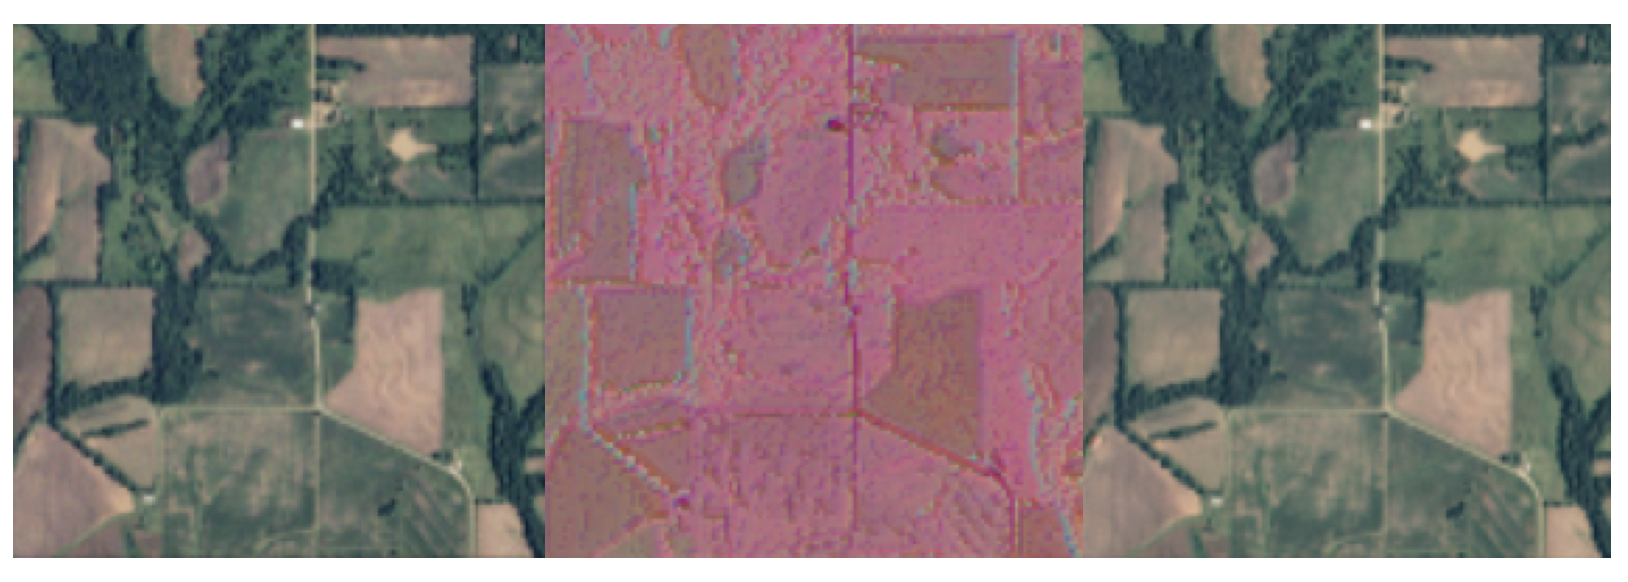
\includegraphics[width=1\linewidth]{images/simon/encLRint_demo.png}
    \begin{justify}
        \textit{Note.} Visualization of an interpolated (left), encoded (middle), and decoded (right) version of the same image. This demonstrates that the AE, even though trained on $HR$ imagery, can accurately process interpolated $LR$ images.
    \end{justify}                    
    \label{fig:encLRint_demo}
\end{figure}



\subsection{Multispectral 20m Band SISR Methodology}
The previous methodologies describe the performance of 4-band RGB-NIR SR on the S2NAIP dataset. To perform SR on the 20m bands of Sentinel-2, certain adaptations are necessary. %First, the synthetic dataset detailed in \autoref{sec:S2NAIP} is utilized.% 

While this dataset does not exactly match the spectral characteristics of the 20m Sentinel-2 bands, it is already adapted between $LR$ and $HR$, spatially co-registered, and degraded using degradation kernels optimized for this task. Since training is performed with random permutations and random ordering of the bands, the models ideally learn the degradation kernels and the spatial frequencies present in the 20m bands, while remaining agnostic to specific bands or values.

A 6-band autoencoder is trained on the described dataset, followed by the training of a 6-band U-Net to perform the actual SR task. These changes necessitate training from scratch.  %The same model descriptions in \autoref{autoencoder}, \autoref{unet}, and \autoref{unet_adaptations} are applicable to the 6-band version. 
While the same spatial features and frequencies apply to both the 10m and 20m bands, they are not interchangeable and must not be used in the same model. The easiest and most efficient approach is to train separate models for each band type, as shown in \autoref{table:sentinel2_bands_model}.


\begin{table}[H]
    \caption{\doublespacing \\ \textit{Model types for the different Sentinel-2 MSI bands.}}
    \begin{spacing}{8}
        \fontsize{8pt}{2pt}\selectfont  
        \begin{tabularx}{\linewidth}{P{6cm}*{4}{c}} 
            \toprule
            \textbf{Band Number} & \textbf{Band Description} & \textbf{Resolution (m)} & \textbf{Model Type} \\
            \midrule
            B1 & Coastal aerosol & 60 & - \\
            B2 & Blue & 10 & 4-band \\
            B3 & Green & 10 & 4-band \\
            B4 & Red & 10 & 4-band \\
            B5 & Vegetation Red Edge & 20 & 6-band \\
            B6 & Vegetation Red Edge & 20 & 6-band \\
            B7 & Vegetation Red Edge & 20 & 6-band \\
            B8 & NIR & 10 & 4-band \\
            B8A & Narrow NIR & 20 & 6-band \\
            B9 & Water Vapor & 60 & - \\
            B10 & SWIR - Cirrus & 60 & - \\
            B11 & SWIR & 20 & 6-band \\
            B12 & SWIR & 20 & 6-band \\
            \bottomrule
        \end{tabularx}
    \end{spacing}
    \vspace{1\baselineskip}
    \textit{Nota.} Model types for the different Sentinel-2 MSI bands.
    \label{table:sentinel2_bands_model}
\end{table}


\section{SISR Training Strategy}
The datasets used in this study and their properties are detailed in \autoref{chapter:datasets}. This section outlines how these datasets are leveraged during the training process for SR models. Due to the high parameter count of the autoencoder and denoising U-Net, large quantities of training data are required. The original authors \autocite{rombach2022highresolution} trained their models using the OpenImages dataset, which contains millions of images. For RGB super-resolution tasks, it is possible to fine-tune the well-optimized checkpoints from these authors using remote sensing imagery. Despite the limited availability of training images in this domain, fine-tuning can be sufficient for this task.

\paragraph{RGB-NIR SISR}
For RGB-NIR SR, training from scratch is required, as no pre-trained models are available for 4-band input. Therefore, large datasets are needed. The following training strategy utilizes different datasets in a sequential manner to take full advantage of their strengths:

\begin{enumerate}
    \item \textit{CV natural images dataset}: This dataset, compiled for this project, contains approximately 280k images. Although it only includes RGB images, we generate the missing fourth band by appending the intensity level of the image as the 4th band. This method is not identical to the NIR band but provides useful spatial and spectral information, as the intensity level is normalized to the same range as the other datasets.
    \item \textit{Sentinel-2 degraded dataset}: Following initial training with natural images, remote sensing data is used. This dataset includes 240k images, although it lacks the spatial properties specific to the research question, as the $LR$ version has a resolution of 40m and the $HR$ version has 10m resolution. However, as it consists of remote sensing images with the same spectral properties as Sentinel-2 data, it helps train the model on relevant spectral and spatial features.
    \item \textit{NAIP dataset}: This dataset closely resembles both the spatial and spectral properties of Sentinel-2 data. The $LR$ version is at 2.5 meters, matching the Sentinel-2 sensor's spectral characteristics, while the $HR$ version is at 2.5m. With 250k images, this dataset alone is sufficient for training from scratch. However, pretraining on previous datasets makes the models more robust.
    \item \textit{Worldstrat dataset}: With only 3k images, this dataset is too small for standalone training or fine-tuning, as the model will overfit. Furthermore, it uses a cross-sensor approach, complicating verification of synthetic results. The final SISR models are not trained on this dataset.
\end{enumerate}

\paragraph{20m-band Multispectral SISR}
The 6-band model follows a similar training strategy. By generating synthetic 6-band S2NAIP datasets, the training process remains consistent through repetition and permutation strategies. The training proceeds as follows:

\begin{enumerate}
    \item \textit{CV natural images dataset}: This dataset serves as the initial training phase, leveraging its abundant data.
    \item \textit{Sentinel-2 degraded dataset}: After pretraining, the model is refined on Sentinel-2 data to focus on satellite-specific image features. However, the interpolation and SR from 80m to 20m introduce challenges with different degradation kernels.
    \item \textit{NAIP dataset}: The 250k images in this dataset serve as the best approximation for the degradation problem at hand, with spatial and spectral similarities making it ideal for training the SR models.
\end{enumerate}

These training strategies enable the 4-band and 6-band models to evolve gradually, moving from a general approach to image reconstruction and SR towards the specific spatial and spectral requirements of the research question.

\subsection{Cross-sensor vs synthetic data}
Various deep learning techniques for super-resolution in earth observation have been proposed \autocite{wang2022review, liu2021research, sdraka2022deep}. These methods are broadly classified into cross-sensor and synthetic approaches. Cross-sensor algorithms require careful spatial alignment and spectral matching of $HR$ and $LR$ pairs, often constrained by the need for large-scale datasets. Synthetic methods, on the other hand, generate $LR$ images by degrading $HR$ images through a blur kernel and downsampling, though domain gaps between synthetic and real-world data remain a challenge \autocite{dong2022real, qiu2023cross, zhang2022single}.
